\section{Application to the Pine Island ice shelf domain}
\label{sec:matern_pig}

Here we show the implementation of the covariance model within the MITgcm,
using the computational grid that we will employ to study the Pine Island cavity
circulation.
We discuss more details on how the grid is obtained in
chapter xx.
However, we mention that the horizontal grid scale is
approximately $\Delta x \simeq \Delta y \simeq 600$~m, and the vertical grid
scale is $\Delta r = 20$~m.
Finally, we note that applying $C$ to a random gaussian vector $\mathbf{z}$
requires the solution to an inverse elliptic operator,
which we obtain with an implementation of a block-Successive Over Relaxation
(SOR) method.
The MITgcm uses no external packages, so interfacing with
e.g.\ \texttt{PETSc} is not an option for any code that is meant to be
contributed to the main MITgcm distribution - which is our intention.
While the solver is far from perfect, it provides decent performance and is
easy to implement.
We discuss details of the implementation and
performance in xx. \\

\noindent\textbf{Samples from the covariance model.}
Figure \ref{fig:matern_samples} (top row) shows samples from the normalized
covariance at the western open boundary of the computational domain,
$XC\mathbf{z}$.
In all cases we use $L_y = 2\Delta y$ and $L_z = \Delta r$, so correlation
length scales vary purely by the specification of $\rangeh$.
The approximate length scale associated with $\rangeh$ is indicated by the arrows on
the bottom right corner of each plot, which qualitatively compares well to the
structure of the random samples.
We note that their is high anisotropy in the domain:
the meridional extent at $Z=0$ (i.e. non-gray distance along the x-axis at the
top of each figure) is $\sim$73~km, while the maximum depth is $\sim1$~km.

The random samples in Figure \ref{fig:matern_samples} (top row)
are normalized by $X$ to have approximately unit variance.
The pointwise marginal standard deviation, $\hat{\sigma}$, which is the inverse
of the diagonal elements of $X$, is shown in Figure \ref{fig:matern_samples}
(bottom row).
With larger correlation length scales, the standard deviation of $C$ increases.
This is particularly true near the boundaries of the field, where we see narrow
bathymetric trenches extending to depth.\\

\begin{figure}
    \centering
    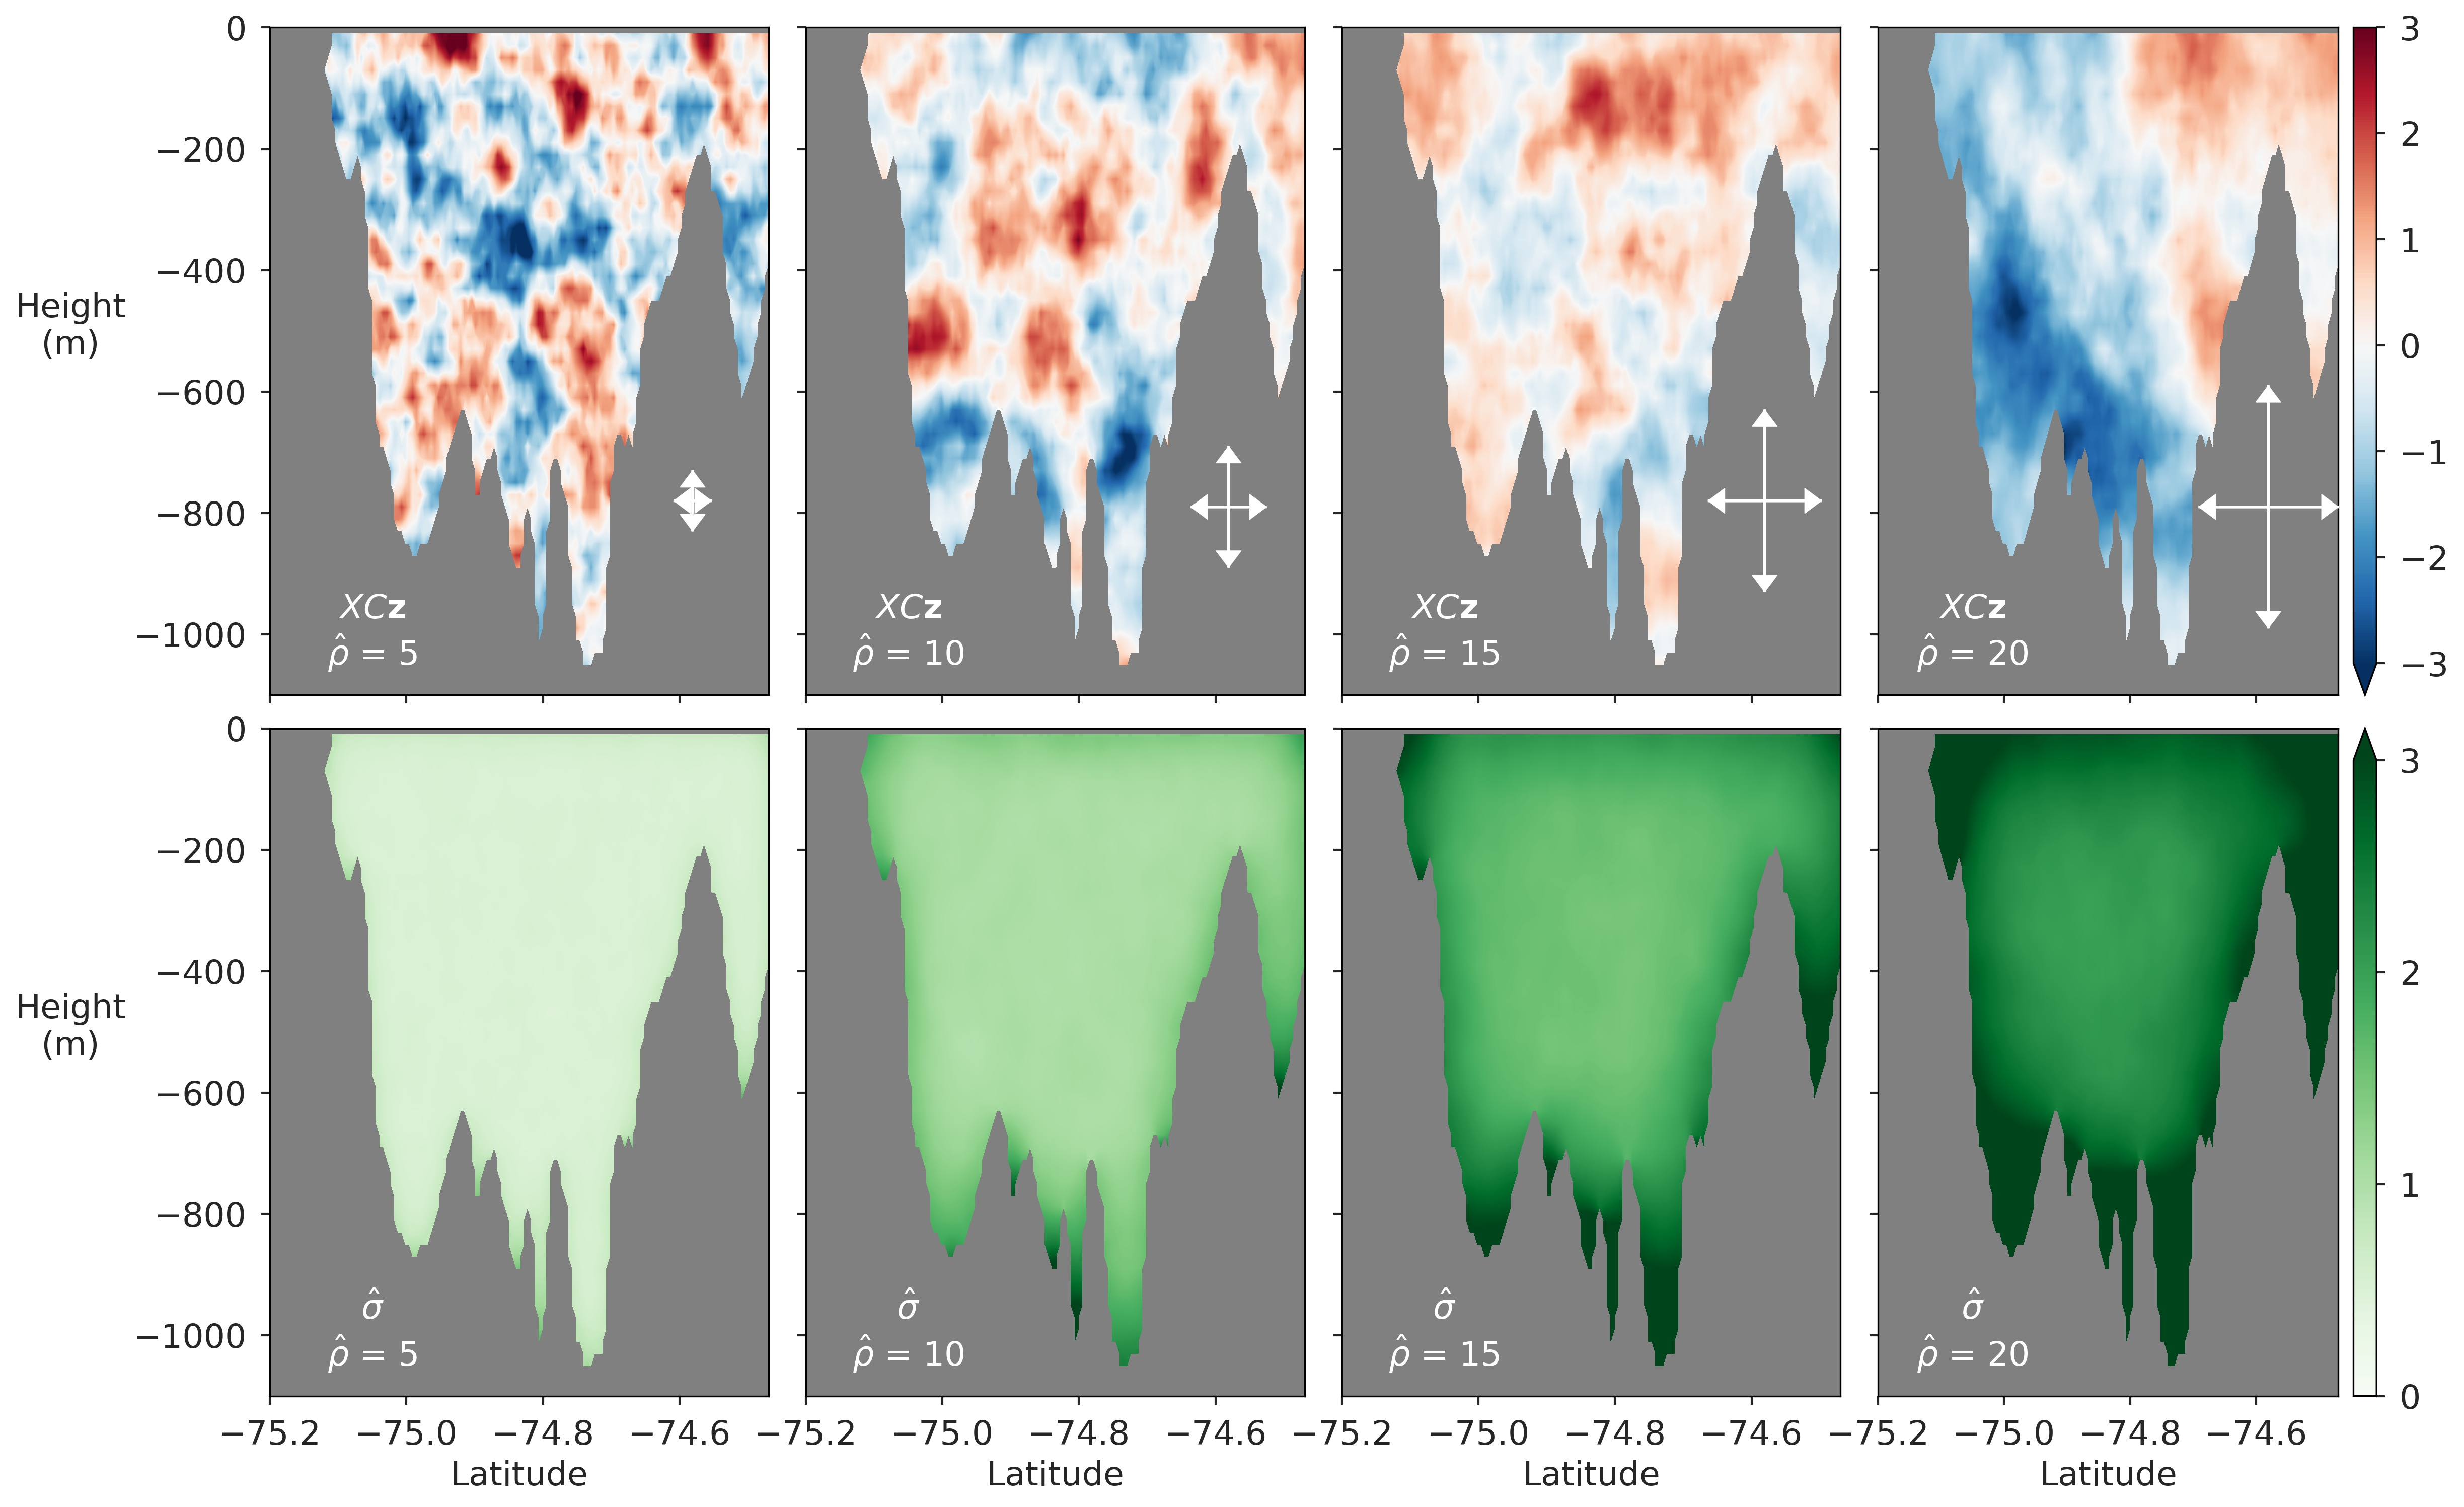
\includegraphics[width=\textwidth]{../figures/samples_and_pointwise_std.jpg}
    \caption{Normalized samples and pointwise standard deviation from the covariance
        model.
        (top row) Samples from the covariance model, normalized by the
        pointwise standard deviation. Each column shows increasing correlation
        length scales, which is regulated by $\rangeh$.
        The arrows in the bottom right corner of each plot show the approximate length scales
        that are covered by $\rangeh L_y$ and $\rangeh L_z$, respectively.
        Here we have used $L_y = 2\Delta y_g$ and $L_z=\Delta r_f$, see
        Figure \ref{fig:mitgcm_grid} for a notational reference.
        We note that the standard normal vector $\mathbf{z}$ is unique in
        each figure.
        (bottom row) Pointwise standard deviation of the covariance operator
        $CC^T$, estimated from
        a sample size of $N=1000$. The diagonal matrix $X$ is comprised of the
        inverse of this field.
    }
    \label{fig:matern_samples}
\end{figure}


\noindent\textbf{Correlation length scales.}
Here we show that the correlations obtained from random samples agree well with
the structure that one would expect from the Mat\'ern model.
We consider the correlation function associated with the isotropic Mat\'ern
covariance from equation \eqref{eq:matern_covariance_iso}:
\begin{linenomath*}\begin{equation*}
    \begin{aligned}
        r(\rangeh,\xh_1,\xh_2) &= r(\rangeh, ||\xh_1-\xh_2||) \\
                       &= c(\xh_1,\xh_2)/\sigma^2 \\
                       &= \dfrac{1}{2^{\meandiff-1}\mathcal{G}(\meandiff)}
        \left(\dfrac{\sqrt{8\meandiff}}{\rangeh} ||\xh_2-\xh_1||\right)^\meandiff
        \mathcal{B}_\meandiff
        \left(\dfrac{\sqrt{8\meandiff}}{\rangeh} ||\xh_2-\xh_1||\right) \, ,
    \end{aligned}
\end{equation*}\end{linenomath*}
which emphasizes that correlation is determined purely by Euclidean distance in
the transformed space.

We compare correlation distances in the computational domain to the
theoretical value, $r(\rangeh,||\xh_1-\xh_2||)$, by using the mapping method described in
section \ref{sec:matern_review}.
Specifically, we compute the correlation coefficient from the random samples
used to approximate $X$ as a function of distance in the computational domain.
We then map these distances back to the ``transformed'' space $\defdomain$ via
the inverse map $\defmap^{-1}$.
We note that $\defmap$ has a differentiable inverse $\defmap^{-1}$ by construction
through the inverse function theorem,
as a result of defining $\defmap$ through its Jacobian $\defjac$ such that
$\defdet \neq 0 \,\,\forall \,\,\x\in\openBdy$.
Specifically, distances in the computational domain are mapped to the
transformed space for arbritrary points $\x_1,\x_2\in\openBdy$ such that
$\xh_1\coloneqq\defmap^{-1}(\x_1)$ and $\xh_2\coloneqq \defmap^{-1}(\x_2)$ as
follows:
\begin{linenomath*}\begin{equation*}
    \begin{aligned}
        \xh_2 - \xh_1 &= \defmap^{-1}(\x_2) - \defmap^{-1}(\x_1) \\
                      &= \left(
                            \defmap^{-1}(\x_1) +
                            \defjac^{-1}\big|_{\x_{1}}(\x_2-\x_1) +
                            \bigo( ||\x_2-\x_1|| )
                        \right) - \defmap^{-1}(\x_1) \\
                        &\simeq \defjac^{-1}\big|_{\x_{1}}(\x_2-\x_1) \, .
    \end{aligned}
    \label{eq:matern_correlation_iso}
\end{equation*}\end{linenomath*}
That is, we use the inverse Jacobian to map distances in the computational domain to the
transformed space $\defdomain$, where we can compare correlation statistics to
the Mat\'ern formula.
We make one final approximation to ease the process.
In the spherical polar coordinate system used, recall that
$\Delta y = r_0 \Delta \phi$, i.e. the meridional grid spacing varies with
latitude.
However, the meridional extent of our computational domain is relatively small,
such that $\Delta y$ only varies from $\sim 582-620$~m.
We therefore assume that
$\defjac^{-1}\big|_{\x_{1}} =\defjac^{-1}\,\,\forall\,\,\x_1\in\openBdy$
simply for the sake of this calculation.

The sample correlation coefficent computed from the 1000 random samples are
shown for various values of $\rangeh$ in Figure \ref{fig:matern_correlations}.
We separately compute distances in the meridional (left panel) and vertical
(right panel) directions as
\begin{linenomath*}\begin{equation*}
    \delta \hat{y} = \defjac^{-1}\delta y
    \qquad
    \delta \hat{z} = \defjac^{-1}\delta z \, .
\end{equation*}\end{linenomath*}
Each colored curve shows the domain averaged correlation coefficient for a
particular $\rangeh$, and the spread denotes one standard deviation above and
below the mean.
Each black curve shows the theoretical, predicted correlation for the distances
in the deformed space $\delta\hat{y}$ and $\delta\hat{z}$.
At larger values of $\rangeh$, the spread in correlation coefficient and
mismatch between the theoretical prediction grow larger.
We attribute this to boundary effects, and note that this slice of the
computational domain has at its maximum extent 60~$L_y$ and 53~$L_z$.
Thus, we expect some degree of difference between the SPDE derived correlation
and the functional form of the covariance model.
However, in general we find the agreement to be quite good.
The result is that we can formulate the covariance model (i.e.\ choose
$\rangeh$) based on our intuition from the simple isotropic form, and this is
easily mapped to the computational domain.

\begin{figure}
    \centering
    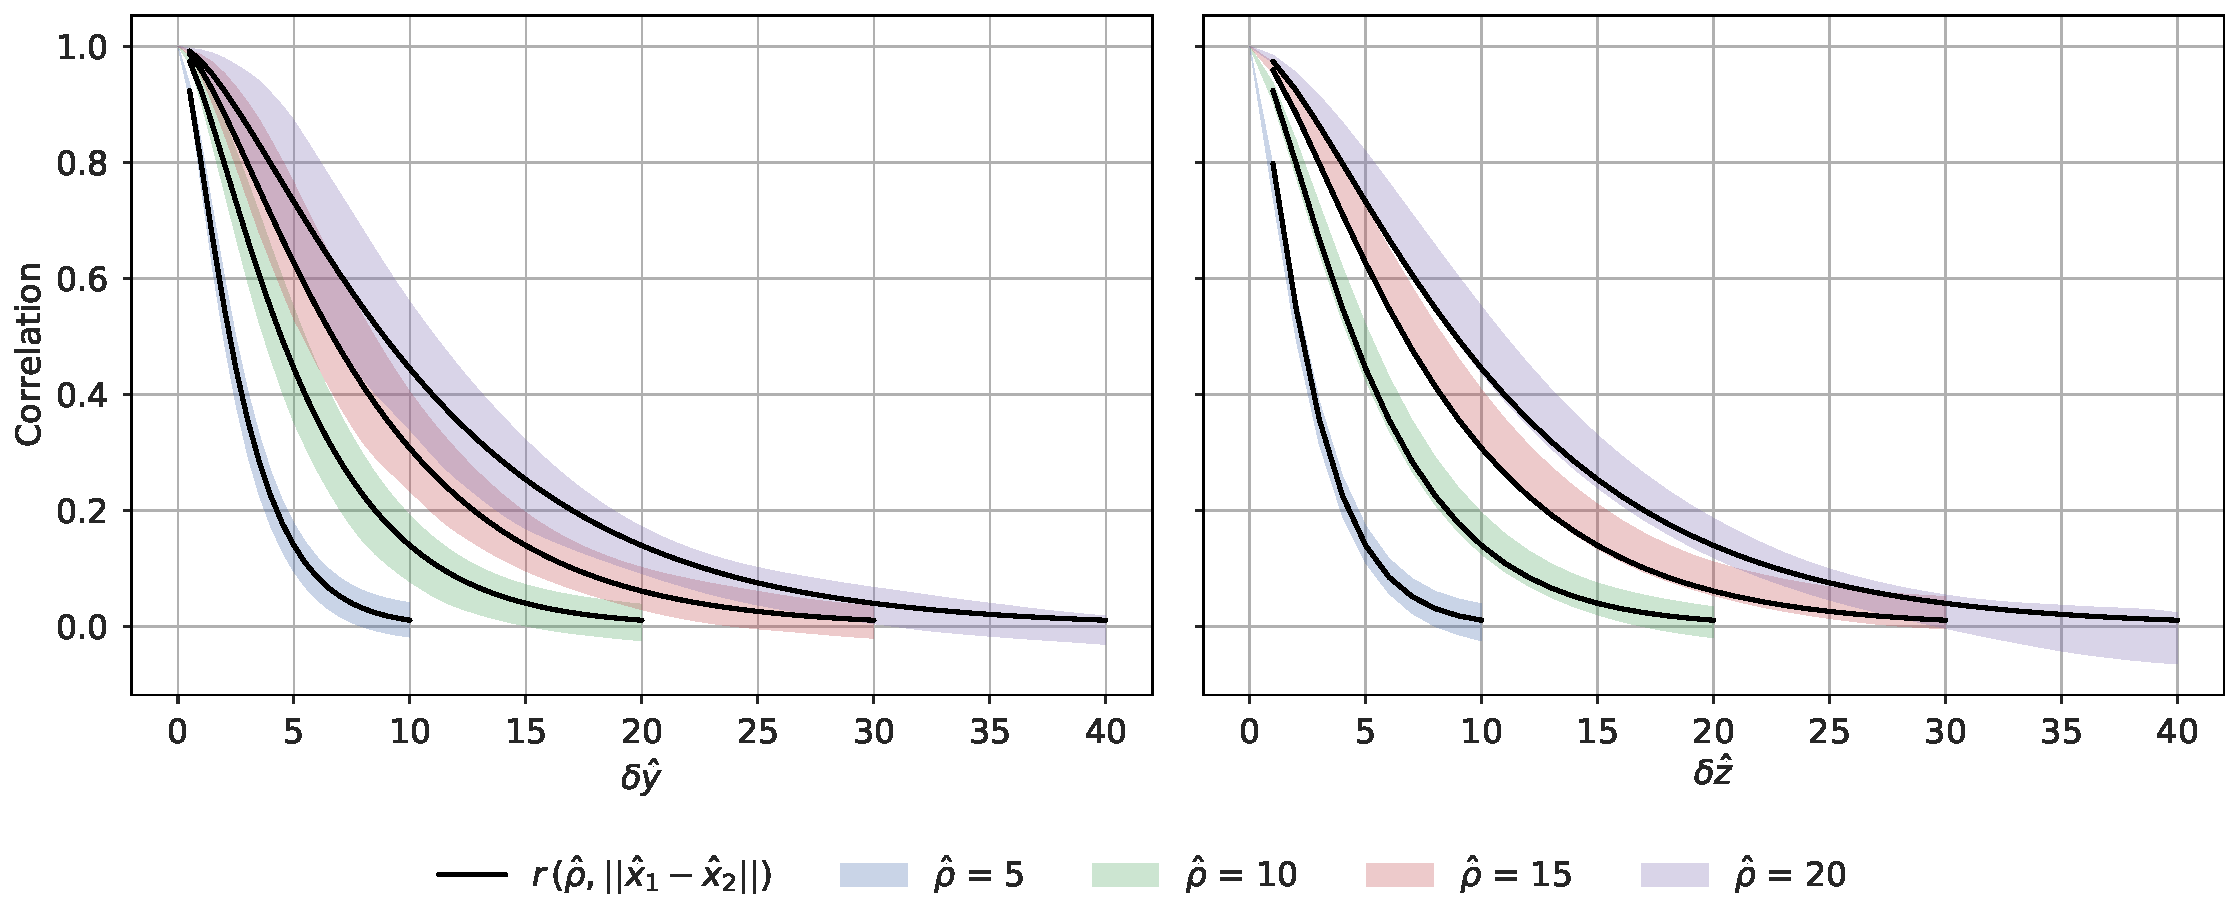
\includegraphics[width=\textwidth]{../figures/nondimensional_correlation.pdf}
    \caption{Correlation coefficient corresponding to different distances in the
        (left) meridional and (right) vertical directions. The coefficient is
        computed from the random samples used to estimate
        $\hat{\sigma}$ and $X$. Each color denotes correlations computed for a
        different value of $\rangeh$, and the spread is determined by one standard
        deviation around the domain averaged correlation coefficent.
        The black curve denotes the predicted isotropic correlation predicted by
        equation \eqref{eq:matern_correlation_iso} with the appropriate value for
        $\rangeh$.}
    \label{fig:matern_correlations}
\end{figure}
